\documentclass[../main.tex]{subfiles}
\usetikzlibrary{calc,trees,positioning,arrows,fit,shapes,calc}

\begin{document}

  \begin{definition}
    $f$ is called \textbf{one-to-one} if $f(x_1) \neq f(x_2)$ whenever $x_1 \neq x_2$ or equivalently
    \[
      f(x_1) = f(x_2) \implies x_1 = x_2
    \]
  \end{definition}

  \begin{figure}[H]
   \centering
   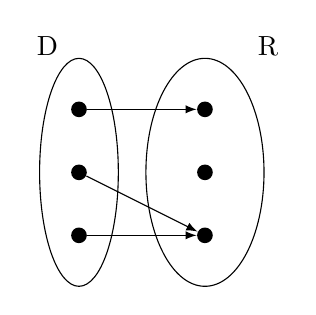
\begin{tikzpicture}[scale=.8]
  %put some nodes on the left
  \foreach \x in {1,2,3}{
  \node[fill,circle,inner sep=2pt] (d\x) at (0,\x) {};
  }
  \node (D) at (-0.5,4) {D};
  \node[fit=(d1) (d2) (d3),ellipse,draw,minimum width=1cm] {};
  %put some nodes on the center
  \foreach \x[count=\xi] in {1,2,3}{
  \node[fill,circle,inner sep=2pt] (r\xi) at (2,\x) {};
  }
  \node (S) at (3,4) {R};
  \node[fit=(r1) (r2) (r3),ellipse,draw,minimum width=1.5cm] {};
  \draw[-latex] (d1) -- (r1);
  \draw[-latex] (d2) -- (r1);
  \draw[-latex] (d3) -- (r3);
\end{tikzpicture}
   \caption{A function which is not 1-1.}
 \end{figure}

 \textbf{Horizontal Line Test.}
 Let $f: \mathbb{R} \to \mathbb{R}$. By definition of a function any vertical line intersects the graph at one point. $f$ is 1-1 if its graph is never intersected by any horizontal line more than once.

 \begin{theorem}
  Increasing or decreasing functions are 1-1.
\end{theorem}

\begin{definition}
  If $f$ is one-to-one then it has an inverse function $f^{-1}$ defined as follows: If $x$ is in the range of $f$ then it is in the domain of $f^{-1}$ and
  \[
    f^{-1}(x) = y \iff x = f(y).
  \]
\end{definition}
If $f$ is not 1-1 then it is not invertible.

Given $y=f(x)$, to find the inverse function, we solve $x$ in terms of $y$.
\begin{example}
  Show that $f(x) = 2x -1$ is one-to-one and find its inverse $f^{-1}(x)$.
\end{example}
\begin{solution}
  Since $f'(x) = 2 >0$, $f$ is increasing on $\mathbb{R}$ and therefore one-to-one for all $x$. Let $y = f^{-1}(x)$, solve for $y$ to get
  \[
    f^{-1}(x) = \frac{x+1}{2}.
  \]
\end{solution}

Usually, we can not solve $y=f(x)$, for example for $y=x+x^3$.

\subsection*{Properties of inverse functions}
\begin{enumerate}
  \item The domain of $f^{-1}$ is the range of $f$.
  \item The range of $f^{-1}$ is the domain of $f$.
  \item $f(f^{-1}(x)) = x$ for all $x$ in the domain of $f^{-1}$.
  \begin{proof}
    If $f^{-1}(x) = y$ then $x = f(y)$ and $f(f^{-1}(x)) = f(y) = x$.
  \end{proof}
  \item $f^{-1}(f(x)) = x$ for all $x$ in the domain of $f$.
  \item $(f^{-1})^{-1}(x) = f(x)$ for all $x$ in the domain of $f$. (The inverse of inverse of $f$ is $f$.)
  \begin{proof}
    \[
      (f^{-1})^{-1}(x) = y \iff f^{-1}(y) = x \iff y = f(x).
    \]
  \end{proof}
  \item The graph of $f^{-1}$ is the reflection of the graph of $f$ in the line $x=y$. (Because if $(a, b)$ is a point on the graph of $y=f(x)$ then $(b, a)$ is a point on the graph of $y = f^{-1}(x)$).
\end{enumerate}
\begin{figure}[H]
  \centering
  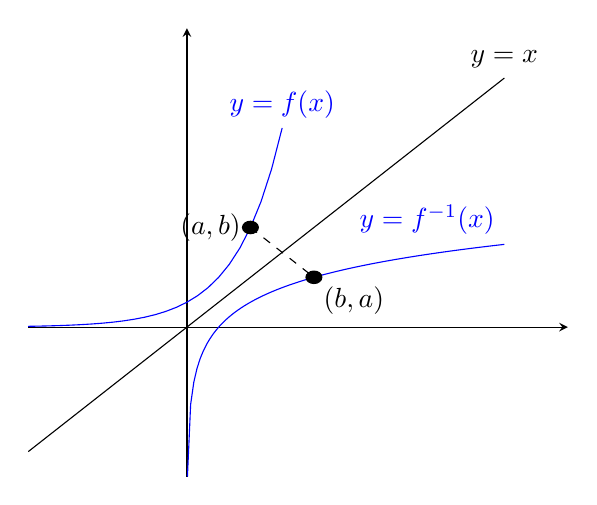
\begin{tikzpicture}
  \begin{axis}[
  xmax=12, ymax=12,
  ticks=none,
  axis lines=middle]
  \addplot[blue, domain=-5:3]  {pow(2,x)} node[above]{$y=f(x)$};
  \addplot[black, domain=-5:10]  {x} node[above]{$y=x$};
  \addplot[blue,domain=1/2^6:10,samples=100]  {log2(x)} node[above left] {$y=f^{-1}(x)$};
  \node [left] at (2,4) {$(a, b)$};
  \draw[fill] (2, 4) circle [radius =0.25];
  \node [below right] at (4,2) {$(b, a)$};
  \draw[fill] (4, 2) circle [radius =0.25];
  \draw[dashed] (2,4) -- (4,2);
\end{axis}
\end{tikzpicture}
  \caption{The graph of the inverse function is a reflection along $y=x$.}
\end{figure}

\subsection*{Inverting Non One-to-one Functions by Restricting the Domain of Definition}
\begin{minipage}{0.5\textwidth}
  The function $f(x) = x^2$ is not one-to-one because $(-a)^2 = a^2$ for any $a$. Hence $f$ is not invertible. Let us define a new function $F$ by restricting the domain of $f$,
  \[
    F(x) = x^2, \quad x \geq 0.
  \]
  Then $F^{-1}(x) = \sqrt{x}$.
\end{minipage}%
\begin{minipage}{0.5\textwidth}
  \begin{figure}[H]
    \centering
    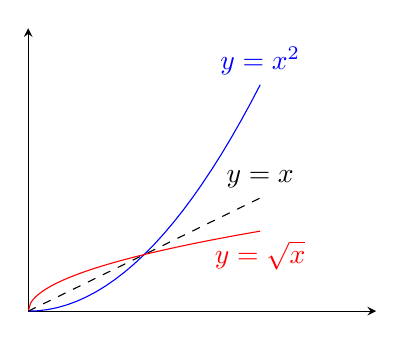
\begin{tikzpicture}
  \begin{axis}[
  width=6cm,
  xmax=3,ymax=5,
  ticks=none,
  axis lines=middle]
  \addplot[blue, domain=0:2]  {x^2} node[above]{$y=x^2$};
  \addplot[red, domain=0:2, samples=100]  {sqrt(x)} node[below]{$y=\sqrt{x}$};
  \addplot[black, dashed, domain=0:2]  {x} node[above]{$y=x$};
\end{axis}
\end{tikzpicture}
    \caption{The restriction of $x^2$ to $[0, \infty)$ and its inverse.}
  \end{figure}
\end{minipage}

Conversely, since the range of the 1-1 function $\sqrt{x}$ is $[0, \infty)$, the domain of its inverse $g(x) = x^2$ is $x\ge0$.
\subsection*{Derivatives of Inverse Functions}

Let $y = f^{-1}(x)$. Then $f(y)=x$. Considering $y$ as a function of $x$ and using implicit differentiation,
\[
  \frac{d}{dx} f(y) = \frac{d}{dx} x \implies f'(y) \frac{dy}{dx} = 1 \implies \frac{dy}{dx} = \frac{1}{f'(y)}
\]
In short if $y=f^{-1}(x)$ then
\[
  (f^{-1})'(x) = \frac{1}{f'(y)} = \frac{1}{f'(f^{-1}(x))}
\]
This formula says if $f'(y) \neq 0$ then $f^{-1}$ is differentiable at $x$.

\begin{figure}[H]
  \centering
  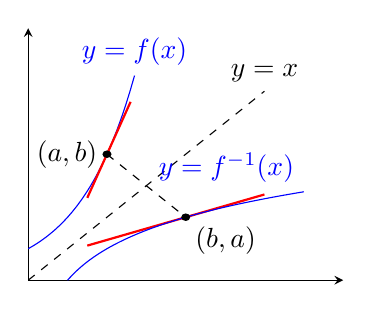
\begin{tikzpicture}
  \begin{axis}[
  xmax=8, ymax=8,
  x=5mm, y=4mm,
  ticks=none,
  axis lines=middle]
  \addplot[blue, domain=0:2.7]  {pow(2,x)} node[above]{$y=f(x)$};
  \addplot[black, domain=0:6, dashed]  {x} node[above ]{$y=x$};
  \addplot[black, domain=1.5:2.6, red, thick]  {4+4*ln(2)*(x-2)};
  \addplot[black, domain=1.5:6, red, thick]  {2+(x-4)/(4*ln(2))};
  \addplot[blue,domain=1:7,samples=100]  {log2(x)} node[above left] {$y=f^{-1}(x)$};
  \node [left] at (2,4) {$(a, b)$};
  \draw[fill] (2, 4) circle [radius =0.1];

  \node [below right] at (4,2) {$(b, a)$};
  \draw[fill] (4, 2) circle [radius =0.1];
  \draw[dashed] (2,4) -- (4,2);
\end{axis}
\end{tikzpicture}
\end{figure}

% A geometric proof that $\tan \theta \tan \beta = 1$. figures/3-1-inversederGeo.eps

In Leibniz notation, $\frac{dy}{dx} = (f^{-1})'(x)$ while $\frac{dx}{dy} = f'(y)$, the above formula reads
\[
  \frac{dy}{dx} \frac{dx}{dy} = 1.
\]

For example, if $y=x^2, x\ge 0$, then $x=\sqrt{y}$ and $\frac{dy}{dx} = 2x$ and $\frac{dx}{dy} = \frac{1}{2\sqrt{y}}$. So
\[
  \frac{dy}{dx} \frac{dx}{dy} = 2x \frac{1}{2\sqrt{y}} = 2x \frac{1}{2x} = 1.
\]
\begin{example}
  Show that $f(x) = x^3 + x$ is one-to-one on the whole real line and find $(f^{-1})'(10)$. Hint: $2^3 + 2 = 10$.
\end{example}
\begin{solution}
  First $f'(x) = 3x^2 + 1 >0$. Hence $f$ is 1-1.
  Let $y = f^{-1}(x)$.
  \[
    (f^{-1})'(x) = \frac{1}{3 y^2 + 1} = \frac{1}{3 (f^{-1}(x))^2 + 1}.
  \]
  \[
    (f^{-1})'(10) = \frac{1}{3 (f^{-1}(10))^2 + 1}.
  \]
  \[
    y = f^{-1}(10) \implies f(y) = 10 \implies y = 2 \implies f^{-1}(10) = 2.
  \]
  Thus
  \[
    (f^{-1})'(10) = \frac{1}{3\times2^2 + 1} = \frac{1}{13}.
  \]
\end{solution}

\begin{example}
  If $f(x) = 3x + x^3$, show that $f$ has an inverse and find the slope of $y=f^{-1}(x)$ at $x=0$.
\end{example}

% \begin{example}[OPTIONAL]
%   Show that
%   \[
%     f(x) =
%     \begin{cases}
%       x^2+1, &\text{ if } x \geq 0\\
%       x+1, &\text{ if } x < 0
%     \end{cases}
%   \]
%   is 1-1 and find its inverse.
% \end{example}
% \begin{solution}
%   $f'(x) > 0$ for $x<0$ and $x>0$ so it is increasing for $x<0$ and $x<0$. Also if $x<0$ then $f(x) < 1 = f(0)$ and if $x>0$ then $1 = f(0) < f(x)$, hence $f$ is increasing everywhere. That proves that $f$ is 1-1.
%   \[
%     f^{-1}(x) =
%     \begin{cases}
%       \sqrt{x-1}, &\text{ if } x \geq 0\\
%       x-1, &\text{ if } x < 0
%     \end{cases}
%   \]
% \end{solution}

\end{document}